\subsection{Basics 1}

\subsubsection{Genders}

French has two grammatical genders: masculine and feminine. All nouns have a gender that you must memorize. Sometimes, the gender can be obvious: une femme ("a woman") is feminine. Other times, it's not obvious: une pomme ("an apple") is also feminine.

\subsubsection{Personal Subject Pronouns}

In every complete sentence, the subject is the person or thing that performs an action or is being described. This is often a noun, but a personal subject pronoun (e.g. "I", "you", or "he") can replace that noun. In both English and French, pronouns have different forms based on what they replace.

\begin{tabular}{lll}
English       & French  & Example                 \\
I             & je      & Je mange. — I eat.      \\
You(singular) & tu/vous & Tu manges. — You eat.   \\
He/It         & il      & Il mange. — He eats.    \\
She/It        & elle    & Elle mange. — She eats.
\end{tabular}

\subsubsection{Subject-Verb Agreement}

Notice above that the verb manger (as well as its English equivalent, "to eat") changes form to agree grammatically with the subject. These forms are called conjugations of that verb. Whenever you want to learn a verb's conjugation, hover your mouse over that word and press the "Conjugate" button. 

\begin{tabular}{|l|l|l|l|}
\hline
\multicolumn{1}{|c|}{\textbf{Subject}} & \multicolumn{1}{c|}{\textbf{Manger (To Eat)}} & \multicolumn{1}{c|}{\textbf{Être (To Be)}} & \multicolumn{1}{c|}{\textbf{Avoir (To Have)}} \\ \hline
je                                     & je mange — I eat                              & je suis — I am                             & j'ai — I have                                 \\ \hline
tu                                     & tu manges — you eat                           & tu es — you are                            & tu as — you have                              \\ \hline
il/elle/on                             & il mange — he eats                            & il est — he is                             & il a — he has                                 \\ \hline
\end{tabular}


\pagebreak
\subsubsection{Articles}

Articles (e.g. "the" or "a") provide context for a noun. In English, articles may be omitted, but French nouns almost always have an article. French has three types of articles:

\begin{itemize}
  \item  Definite articles ("the") are used with specific nouns that are known to the speakers, as in English, but also to indicate the general sense of a noun, unlike in English.
  \item  Indefinite articles ("a"/"an"/"one") are used for countable nouns that are unspecified or unknown to the speakers.
  \item  Partitive articles ("some"/"any") indicate a quantity of something uncountable.
\end{itemize}
    
Articles have multiple forms, as provided in this table:

\begin{tabular}{|r|l|l|l|l|}
\hline
\multicolumn{1}{|l|}{\textbf{Article}} & \multicolumn{1}{c|}{\textbf{Masculine}} & \multicolumn{1}{c|}{\textbf{Feminine}} & \multicolumn{1}{c|}{\textbf{Plural}} & \multicolumn{1}{c|}{\textbf{Example}} \\ \hline
\textbf{Definite}                      & le/l'                                   & la/l'                                  & les                                  & le chat — the cat                     \\ \hline
\textbf{Indefinite}                    & un                                      & une                                    & des                                  & une femme — a woman                   \\ \hline
\textbf{Partitive}                     & du/de l'                                & de la/de l'                            &                                      & de l'eau — (some) water               \\ \hline
\end{tabular}

It is critical to understand that articles must agree with their nouns in both gender and number. For instance, le femme is incorrect. It must be la femme because la is feminine and singular, just like femme.

\subsubsection{Elisions}

Le and la become just l' if they're followed by a vowel sound. This is an example of \textit{elision}, which is the removal of a vowel sound in order to prevent consecutive vowel sounds and make pronunciation easier. Elisions are mandatory---for instance, ``je aime'' is incorrect. It must be ``j'aime''.

These other one-syllable words can also elide: je, me, te, se, de, ce, ne, and que. Tu can also be elided in casual speech, but not in writing (including on Duolingo).

\subsubsection{Contractions}

In a contraction, two words combine to form one shortened word. For instance, the partitive article du is a contraction of the preposition de with le.

\begin{itemize}
  \item  du pain — (some) bread
\end{itemize}
    
However, since du can create vowel conflicts, when it would appear in front of a vowel sound, it takes the elided de l' form instead. This is also the case for de la.
\begin{itemize}
  \item  de l'ananas [masc.] — (some) pineapple
  \item  de l'eau [fem.] — (some) water
\end{itemize}

\subsubsection{Words Beginning with H}

The letter H is always mute (silent) in French, but when H starts a word, it can act as a consonant (aspirate) or vowel (non-aspirate). For example, the H in homme acts as a vowel. This means that "the man" must be written as l'homme.  Conversely, an aspirate H doesn't participate in elisions or liaisons (which you'll learn about soon). It's usually found at the beginning of loanwords from German or other languages. For instance, "the hero" is le héros. Pay attention to this when learning new vocabulary.


\pagebreak
\subsubsection{First Vocabulary}

\begin{center}\begin{tabular}{l|l||l|l}
\textbf{French} & \textbf{English} & \textbf{French} & \textbf{English} \\ \hline
\Red{la femme} & woman  & il & he \\
\Red{la fille} & girl & \Blue{le chat} & cat \\
\Blue{le gar\c con} & boy & noir & black \\
\Blue{l'homme} & man & \Red{la robe} & dress \\
\Red{la pomme} & apple & et & and \\
\Red{l'orange} & orange & calme & calm \\
l'enfant & child & riche & rich \\
elle & she \\
\end{tabular}\end{center}

\begin{itemize}
  \item  Je suis rouge! \\ I am red!
\end{itemize}


\pagebreak
\subsection{Basics 2}

\subsubsection{Plurals}

Many French words have plural forms. Plural nouns and adjectives often end in -s, though the S is usually silent.

\begin{itemize}
  \item  homme ("man") $\Rightarrow$ hommes ("men")
  \item  femme ("woman") $\Rightarrow$ femmes ("women")
  \item  chat noir ("black cat") $\Rightarrow$ chats noirs ("black cats")
\end{itemize}

There are also plural forms for pronouns and verb conjugations. Consider parler ("to speak"):

\begin{center}
\begin{tabular}{|r|c|l|}
\hline
\textbf{Person}                   & \textbf{French} & \textbf{Example}             \\ \hline
I                                 & je              & Je parle. $\Rightarrow$ I speak.         \\ \hline
You (singular)                    & tu              & Tu parles. $\Rightarrow$ You speak.      \\ \hline
You (formal)                      & vous            & Vous parlez. $\Rightarrow$ You speak.    \\ \hline
He                                & il              & Il parle. $\Rightarrow$ He speaks.       \\ \hline
She                               & elle            & Elle parle. $\Rightarrow$ She speaks.    \\ \hline
We                                & nous            & Nous parlons. $\Rightarrow$ We speak.    \\ \hline
You (plural)                      & vous            & Vous parlez. $\Rightarrow$ You speak.    \\ \hline
They (any group including a male) & ils             & Ils parlent. $\Rightarrow$ They speak.   \\ \hline
They (all women)                  & elles           & Elles parlent. $\Rightarrow$ They speak. \\ \hline
\end{tabular}
\end{center}

\subsubsection{Tu or Vous?}

French has two words for the subject pronoun "you": tu and vous. For a singular "you", tu should only be used for friends, peers, relatives, children, or anyone else who's very familiar to you. In all other cases and also for plurals, the more polite vous should be used to show respect. When in doubt, use vous.

\subsubsection{Agreement}

Pronouns, adjectives, and articles must agree with their nouns in both gender and number. Consider the examples below and note how the article and adjective change to agree with each noun.

\begin{itemize}
  \item  Masculine singular: Le chat noir $\Rightarrow$ The black cat
  \item  Masculine plural: Les chats noirs $\Rightarrow$ The black cats
  \item  Feminine singular: La robe noire $\Rightarrow$ The black dress
  \item  Feminine plural: Les robes noires $\Rightarrow$ The black dresses
\end{itemize}

Not all adjectives change forms. For instance, riche is the same for both masculine and feminine singular nouns.

\subsubsection{Continuous Tenses}

English has two present tenses: simple ("I write") and continuous ("I am writing"), but French has no specialized continuous verb tenses. This means that "I write", "I am writing", and "I do write" can translate to j'écris (not je suis écris) and vice versa.  However, the idiomatic phrase « être en train de » is often used to indicate that someone is in the process of doing something.

\begin{itemize}
  \item  Je suis en train de manger. — I am [in the process of] eating.
\end{itemize}
    
When translating, remember that English stative verbs have no continuous forms. For instance, « j'aime un garçon » cannot be translated as "I am loving a boy".

\subsubsection{L'Amour}

Love is tricky in France. For people and pets, aimer means "to love", but if you add an adverb, like in aimer bien, it means "to like". For everything else, aimer only means "to like". Adorer can always mean "to love", though it tends to be more coy than aimer.

\subsubsection{Vocabulary}

\begin{center}\begin{tabular}{l|l||l|l}
\textbf{French} & \textbf{English} & \textbf{French} & \textbf{English} \\ \hline
\Red{la lettre} & letter & \Blue{le journal} & newspaper \\
\Red{la robe} & dress & \Blue{le menu} & menu \\
\end{tabular}\end{center}


\pagebreak
\subsection{Phrases}

\subsubsection{Bonjour!}

Bonjour is a universal greeting that can be spoken to anyone at any time. In France, greeting people is very important, and some will even say bonjour aloud when entering a public room or bus. Bon après-midi is often used as a farewell in the afternoon, while bonsoir is an evening greeting.

\begin{itemize}
  \item  Greetings: bonjour, bonsoir (plus bon matin in Québec only)
  \item  Farewells: bonne journée, bon après-midi, bonne soirée, bonne nuit
\end{itemize}

\subsubsection{Idioms}

Many words or phrases cannot be translated literally between English and French because their usages are idiomatic. For instance, consider ``Ça va ?'', which means ``How are you?'' The literal translation of the French is ``That goes?'', but this is nonsensical in English. It is very important to identify idioms in both languages and learn how to translate them properly.

\begin{center}
  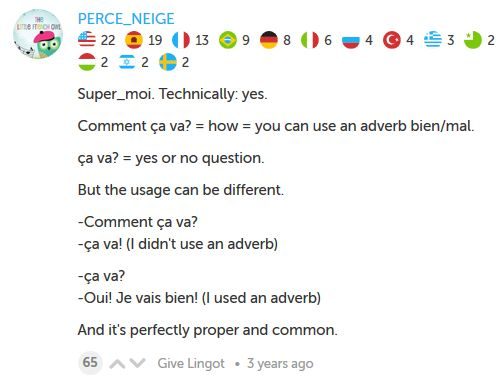
\includegraphics[scale = 0.5]{images/cava.jpg}
\end{center}

\subsubsection{Liaisons}

In a liaison, an otherwise silent ending consonant is pushed to the next word, where it's pronounced as part of the first syllable. Like elisions, this prevents consecutive vowel sounds. Liaisons are possible whenever a silent ending consonant is followed by a word beginning in a vowel sound, but some liaisons are mandatory and others are forbidden.  Here are some mandatory liaisons, along with approximate pronunciations:

\begin{itemize}
  \item  Articles and adjectives with nouns. For example, un homme ("uh-nohm") \\ mon orange ("mohn-norahnge"), or deux hommes ("duh-zohm").
  \item  Pronouns and verbs. For example, nous allons ("noo-zalohn") or est-il ("ay-teel").
  \item  Single-syllable adverbs and prepositions. For instance, très utile ("tray-zuteel") or chez elle ("shay-zell").
\end{itemize}

Liaisons that are forbidden:

\begin{itemize}
  \item  Before and after et ("and").
  \item  After singular nouns (including proper nouns and names).
  \item  After inversions (which you'll learn in "Questions").
  \item  Before an aspirated H (e.g. héros - "hero").
  \item  After a nasal sound, except that un, on, and en do liaise.
\end{itemize}

Note that some consonants take on a different sound in liaisons, and it's important to pronounce these correctly when speaking.\footnote{Liaison rules vary among speakers, particularly across dialects, and fewer liaisons tend to appear in casual and slow speech. Note that the slow mode in Duo listening exercises does not include liaisons.}

\begin{center}\begin{tabular}{|c|c|c|}
\hline
\textbf{Original Consonant} & \textbf{Resulting Liaison Sound} & \textbf{Example}                    \\ \hline
-s, -x, -z                  & Z                                & des hommes ("day-zohm")             \\ \hline
-d                          & T                                & un grand arbre ("uhn-grahn-tarbre") \\ \hline
-f                          & V                                & neuf ans ("nuh-vahn")               \\ \hline
\end{tabular}\end{center}

\subsubsection{Encha{\^i}nement}

In encha{\^i}nements, ending consonant sounds are pushed onto the next word if it begins in a vowel. This is essentially the same as a liaison, except that the consonant sound wasn't silent beforehand. For instance:

\begin{itemize}
  \item  elle est is pronounced like "eh-lay".
  \item  mange une pomme is pronounced like "mahn-jun-pom".
\end{itemize}

\subsubsection{The Impersonal Expression Il Y A}

Impersonal expressions are phrases where there isn't a real subject. For instance, in the phrase "It is snowing" (Il neige), "it" doesn't refer to anything. It's a dummy subject that exists just to maintain the sentence structure.  One of the most common impersonal expressions is il y a, which is an idiom for "there is" or "there are".

\begin{itemize}
  \item  Il y a une fille ici. \\ There is a girl here.
  \item  Il y a un serpent dans ma botte ! \\ There's a snake in my boot!
\end{itemize}

\subsubsection{Vocabulary}

\begin{center}\begin{tabular}{l|l||l|l}
\textbf{French} & \textbf{English} & \textbf{French} & \textbf{English} \\ \hline
oui & yes & {\c c}a va & how are you? \\
non & no & comment {\c c}a va & how are you? \\
s'il vous pla{\^i}t & please & {\c C}a va bien & I am well. \\
merci & thank you & pardon & pardon me \\
merci beaucoup & thank you very much & d{\' e}sol{\' e} & sorry \\
bonjour & hello & Bienvenue! & Welcome! \\
bonsoir & good evening & {\`A} bient{\^o}t! & See you soon! \\
salut & bye & {\`A} plus tard! & See you later! \\
au revoir & goodbye & {\`A} demain! & See you tomorrow! \\
bonne nuit & good night & D'accord & Okay \\
\end{tabular}\end{center}

\begin{itemize}
  \item  Oui, je suis d{\' e}sol{\' e}. \\ Yes, I am sorry.
\end{itemize}


\pagebreak
\subsection{Food}

\subsubsection{The Partitive Article}

The partitive article is used for unspecified amounts of uncountable nouns. In English, it can translate to "some", but it's often just omitted. Remember that du is a contraction of de + le and that partitives can elide.

\begin{center}\begin{tabular}{|c|c|c|}
\hline
\textbf{Gender} & \textbf{Partitive Article} & \textbf{Example}                               \\ \hline
Masculine       & du                         & Je mange du poisson. — I am eating fish.       \\ \hline
Feminine        & de la                      & Je mange de la viande. — I am eating meat.     \\ \hline
Elided Masc.    & de l'                      & Je mange de l'ananas. — I am eating pineapple. \\ \hline
Elided Fem.     & de l'                      & Je bois de l'eau. — I am drinking water.       \\ \hline
\end{tabular}\end{center}

Nouns almost never appear without articles in French, so articles must be repeated in serial lists.  For example,

\begin{itemize}
  \item  Il cuisine du poisson et de la viande \\ He cooks fish and meat.
\end{itemize}

\subsubsection{Count Noun, Mass Noun, or Both?}

\textbf{Count nouns} are discrete and can be counted, like un livre ("a book"). They can be modified by definite and indefinite articles, but not partitive articles.

\begin{itemize}
  \item  Je lis un livre. \\ I am reading a book.
  \item  Nous avons les livres. \\ We have the books.
\end{itemize}

\textbf{Mass nouns} like lait ("milk") are uncountable, and they can be modified by definite and partitive articles, but not indefinite articles.

\begin{itemize}
  \item  Je bois du lait. \\ I am drinking [some] milk.
  \item  Je bois le lait. \\ I am drinking the milk.
\end{itemize}

However, many nouns can behave as both count nouns and mass nouns. This is true for most edible things. For instance, consider poisson ("fish") or vin ("wine"):

\begin{itemize}
  \item  Count noun: Le poisson est rouge. \\ The fish is red.
  \item  Mass noun: Je mange du poisson. \\ I eat [some] fish.
  \item  Count noun: Le vin est blanc. \\ The wine is white.
  \item  Mass noun: Je bois du vin rouge ou blanc. \\ I drink red or white wine.
\end{itemize}

Note that some mass nouns can be pluralized in English when they refer to multiple types of the noun, but this usage isn't found in French. For instance, "the fishes" refers to multiple species of fish, while les poissons just refers to multiple fish.

\subsubsection{Omitted Articles}

When an article is missing in an English sentence, it must be added to the French translation. The definite article can be used to fill this void in three situations:

\begin{itemize}
  \item  Almost anywhere one would use "the" in English (i.e. when referring to specific things).
  \item  Before the subject of a sentence to state general truths about it.
  \item  Before the direct object of a verb of appreciation (like aimer) to express like/dislike.
\end{itemize}

If any of the above is true, then use the definite article. Otherwise, use the indefinite or partitive, depending on whether or not the noun is countable.

\begin{itemize}
  \item  I like wine, but I am drinking milk. \\ J'aime le vin, mais je bois du lait.
\end{itemize}

Both articles are missing in the English version of this example. Aimer expresses fondness for wine, so le vin should be used there. However, boire is not a verb of appreciation, so the partitive du should be used on the uncountable lait.

\begin{itemize}
  \item  Cats are animals. \\ Les chats sont des animaux.
\end{itemize}

This is a general truth about cats, but (2) above can only apply to subjects, so only chats takes a definite article here. Animaux are countable, so use the plural indefinite des.

\begin{itemize}
  \item  He likes to eat meat. \\ Il aime manger de la viande.
\end{itemize}

This is a tricky example because the meat is the direct object of manger, not aimer. Thus, (3) does not apply and viande cannot take a definite article.  Also, the French definite article can be ambiguous when translating from French to English. It can often refer to both a specific noun and the general sense of a noun.

\begin{itemize}
  \item  Les chats sont des animaux. \\ Cats are animals. / The cats are animals.
\end{itemize}
    
\subsubsection{De + Definite Article}

De plus a definite article can also have other meanings. De means "of" or "from", so this can also indicate possession or association with a definite noun.

\begin{itemize}
  \item  La copie du livre. \\ The copy of the book.
  \item  Les copies des livres. \\ The copies of the books.
  \item  L'enfant de la femme. \\ The woman's child.
\end{itemize}

\subsubsection{Vocabulary}

\begin{center}\begin{tabular}{l|l||l|l}
\textbf{French} & \textbf{English} & \textbf{French} & \textbf{English} \\ \hline
boivent & to drink & \Blue{le repas} & meal \\
mangent & to eat & \Red{la boisson} & beverage \\
cuisine & to cook & \Blue{le th{\'e}} & tea \\
\Blue{le sandwich} & sandwich & \Red{la cr{\^e}pe} & crepe \\
\Red{la tomate} & tomato & \Blue{le beurre} & butter \\
\Red{la soupe} & soup & \Blue{le fromage} & cheese \\
\Red{la fraise} & strawberry & \Blue{le poisson} & fish \\
\Red{la viande} & beef & \Blue{le bonbon} & candy \\
\Red{la baguette} & baguette & \Red{la banane} & banana \\
\Blue{le oignon} & onion & \Blue{le sel} & salt \\
l'eau & water & \Blue{le poivre} & pepper \\
l'{\oe}uf & egg & \Blue{le sucre} & sugar \\
l'alcool & alcohol & \Blue{le poulet} & chicken \\
\Red{la salade} & salad & \Blue{le porc} & pork \\
\Blue{le riz} & rice & \Blue{le g{\^a}teau} & cake \\
\Red{la bi{\`e}re} & beer & \Blue{le citron} & lemon \\
\Blue{le lait} & milk & \Blue{le chocolat} & chocolate \\
\Blue{le pain} & bread & \Blue{le b{\oe}uf} & beef \\
\Blue{le vin} & wine & \Blue{le raisin} & grape \\
\Blue{le caf{\'e}} & coffee & \Blue{le jus} & juice \\
avec & with \\
\end{tabular}\end{center}

\begin{itemize}
  \item  Je bois de la bi{\`e}re. \\ I drink beer.
  \item  Les hommes mangent du fromage. \\ The men drink beer.
  \item  Nous avons du sucre. \\ We have sugar.
\end{itemize}


\pagebreak
\subsection{Animals}

\subsubsection{Noun Genders}

One of the most difficult aspects of learning French is memorizing noun genders. However, by spending some time now memorizing the following patterns, you may be able to guess most nouns' genders and save yourself a lot of trouble in the future.  Some nouns, like l'élève ("the student"), have the same spelling and meaning in both forms. Other nouns have the same spelling, but have different meanings. Un tour is a tour, while une tour is a tower. There are also nouns that only have one possible gender. Even a baby girl is un bébé, for instance. Many masculine nouns can be changed to a feminine form simply by adding an -e to the end. Your male friend is un ami and your female friend is une amie.  Some genders depend on a noun's classification. For instance, languages, days of the week, months, seasons, metals, colors, and measurements are mostly masculine.  Otherwise, memorizing word endings is the best way to guess genders. We'll learn these ending patterns in four steps:

\begin{enumerate}
  \item  Nouns ending in -e tend to be feminine. All others, especially nouns ending in consonants, tend to be masculine. This is true for over 70\% of all nouns.
  \item  Nouns that have the endings -ion and -son tend to be feminine, even though they end in consonants.
  \item  Nouns with these endings are usually masculine, although they end in -e:
    \begin{itemize}
      \item  -tre, -ble, -cle (think "treble clef")
      \item  -one, -ème, -ège (think "OMG")
      \item  -age, -isme
    \end{itemize}
  \item  Watch out for these complications:
    \begin{itemize}
      \item  -é is masculine, but -té is feminine. \\ le résumé (masc) — the resumé \\ la liberté (fem) — the liberty
      \item  -de is masculine, but -ade, -nde, and -ude are feminine. \\ le guide — the guide \\ la parade — the parade
      \item  -ste and -me tend to be masculine, but there are dozens of exceptions. Words for people ending in -ste are often gender-neutral, e.g. le/la cycliste.
      \item  -eur is masculine for most professions or technical terms, but it's feminine for some emotions and abstract things. \\ le chauffeur — the driver \\ la peur — the fear
    \end{itemize}
\end{enumerate}

That's it! Memorize these, and you'll be able to guess most noun genders.

\subsubsection{Feminine Animals}

In French, female animal nouns are generally formed as follows by taking the last consonant, doubling it, and adding a mute -e to the end.

\begin{itemize}
  \item  un chat $\quad\Rightarrow\quad$ une chatte
  \item  un chien $\quad\Rightarrow\quad$ une chienne
\end{itemize}

Of course, there are many exceptions. For example:

\begin{itemize}
  \item  un ours $\quad\Rightarrow\quad$ une ourse (not une oursse)
  \item  un cheval $\quad\Rightarrow\quad$ une jument (not une chevalle)
\end{itemize}

\subsubsection{Vocabulary}

\begin{center}\begin{tabular}{l|l||l|l}
\textbf{French} & \textbf{English} & \textbf{French} & \textbf{English} \\ \hline
\Purple{cheval} & horse & \Blue{le singe} & monkey \\
\Purple{chien} & dog & \Purple{requin} & shark \\
\Blue{l'animal} & animal & \Red{l'abeille} & bee \\
\Blue{l'oiseau} & bird & \Purple{serpent} & snake \\
\Purple{canard} & duck & \Blue{l'araign{\'e}e} & spider \\
\Purple{chat} & cat & \Red{la souris} & mouse \\
\Purple{l'{\'e}l{\'e}phant} & elephant & \Blue{le papillon} & butterfly \\
\Purple{ours} & bear & \Blue{l'insecte} & insect \\
\Red{la tortue} & turtle & \Red{la fourmi} & ant \\
\Purple{lion} & lion & \Red{la baleine} & whale \\
\Red{la vache} & cow & \Blue{le dauphin} & dolphin \\
\Purple{cochon} & pig & \Blue{le loup}, \Red{la louve} & wolf \\
\Red{la mouche} & [house]fly & \Purple{lapin} & rabbit \\
\Blue{le tigre} & tiger & \Red{la poule} & hen \\
\end{tabular}\end{center}


\pagebreak
\subsection{Adjectives}

Unlike English adjectives, French adjectives must agree in number and gender with the nouns that they modify. A black dog is un chien noir, but a black dress is une robe noire. Also, remember that some adjectives have the same masculine and feminine form, especially those ending in a silent -e (e.g. riche).  When used with pronouns, adjectives agree with the noun that has been replaced. This is particularly tricky with the formal vous: to a singular man, you would say vous êtes beau, but to plural women, you would say vous êtes belles.

\subsubsection{Adjective Placement}

In French, most adjectives appear after the nouns they modify. For instance, le chat noir. However, some adjectives precede the noun. You can remember these types of nouns using the mnemonic \Purple{BANGS}.

\begin{itemize}
  \item  \Purple{B} is for beauty. Une belle femme $\quad\Rightarrow\quad$ A beautiful woman
  \item  \Purple{A} is for age. Une jeune fille $\quad\Rightarrow\quad$ A young girl
  \item  \Purple{N} is for number.\footnote{This can also be for rank: Le premier mot — The first word} Deux hommes $\quad\Rightarrow\quad$ Two men
  \item  \Purple{G} is for good or bad. Un bon garçon $\quad\Rightarrow\quad$ A good boy
  \item  \Purple{S} is for size. Un gros chat $\quad\Rightarrow\quad$ A fat cat
\end{itemize}

All determiner adjectives (e.g. possessives, interrogatives, and demonstratives) appear before the noun, e.g. mon livre ("my book") and ce cochon ("that pig"). You will learn these later.

\subsubsection{Figurative Adjectives}

A few adjectives can come both before and after the noun depending on their meaning. The most common example is grand, which is a BANGS adjective for everything but people. For people, it comes before a noun when it means "important" and after the noun when it means "tall". For instance, Napoleon was un grand homme ("a great man"), but not un homme grand ("a tall man").  Usually, figurative meanings will precede the noun, while literal meanings will follow the noun.

\begin{itemize}
  \item  un pauvre homme $\quad\Rightarrow\quad$ a pitiful man
  \item  un homme pauvre $\quad\Rightarrow\quad$ a poor man
  \item  un certain nombre $\quad\Rightarrow\quad$ a certain (particular) number
  \item  une victoire certaine $\quad\Rightarrow\quad$ a certain (guaranteed) victory
  \item  ma propre voiture $\quad\Rightarrow\quad$ my own car
  \item  ma voiture propre $\quad\Rightarrow\quad$ my clean car
  \item  un cher ami $\quad\Rightarrow\quad$ a dear friend
  \item  une montre chère $\quad\Rightarrow\quad$ an expensive watch
\end{itemize}

\subsubsection{Euphony}

As you have already learned, elisions, contractions, liaisons, and enchaînements are all designed to prevent consecutive vowel sounds (which is called hiatus). This quest for harmonious sounds is called euphony and is an essential feature of French. It has, however, created some unexpected rules.  For instance, the masculine beau ("beautiful") changes to bel if its noun begins with a vowel sound. A beautiful man is un bel homme. The other two common changes are vieux to vieil ("old") and nouveau to nouvel ("new").  Note that this doesn't occur to feminine adjectives because they usually end in silent vowels.
    
\subsubsection{Vocabulary}

\begin{center}\begin{tabular}{l|l||l|l}
\textbf{French} & \textbf{English} & \textbf{French} & \textbf{English} \\ \hline
froid & cold & grand & large \\
chaud & hot & jeune & young \\
nouveau & new & joil & pretty \\
petit & small \\
\end{tabular}\end{center}


\pagebreak
\subsection{Plurals}

Most plural forms of nouns and adjectives can be formed by appending an -s to the singular, but remember that this -s is usually silent.

\begin{itemize}
  \item  Le chat noir $\quad\Rightarrow\quad$ The black cat $\quad\Rightarrow\quad$ Les chats noirs $\quad\Rightarrow\quad$ The black cats
  \item  Un chat noir $\quad\Rightarrow\quad$ A black cat $\quad\Rightarrow\quad$ Des chats noirs $\quad\Rightarrow\quad$ (Some) black cats
\end{itemize}

Note: If the noun is preceded by an adjective, des becomes de.

\begin{itemize}
  \item  Un petit chat $\quad\Rightarrow\quad$ A little cat $\quad\Rightarrow\quad$ De petits chats
\end{itemize}

Articles must agree with the nouns they modify, so plural nouns require either les or des. This is a great way to tell if a noun is plural. If you hear les or des (which sound similar to "lay" and "day"), then the noun is plural. If not, it's probably singular.  Remember that verbs change conjugation to agree with their subjects in both grammatical person and number.

\begin{center}\begin{tabular}{|r|c|l|}
\hline
\textbf{Subject}    & \textbf{{\^E}tre ("to be")} & \textbf{Parler ("to speak")} \\ \hline
\textbf{je}         & suis                    & parle                        \\ \hline
\textbf{tu}         & es                      & parles                       \\ \hline
\textbf{il/elle/on} & est                     & parle                        \\ \hline
\textbf{nous}       & sommes                  & parlons                      \\ \hline
\textbf{vous}       & {\^e}tes                & parlez                       \\ \hline
\textbf{ils/elles}  & sont                    & parlent                      \\ \hline
\end{tabular}\end{center}

\subsubsection{Punctuation}

There are no quotation marks in French. Instead, the French use guillemets (\guillemotleft \guillemotright). Exclamation marks (!), question marks (?), colons (:), semicolons (;) and guillemets need to have a space on either side.

\begin{itemize}
  \item  Incorrect: ``{\c C}a va?''
  \item  Correct: \guillemotleft~{\c C}a va ? \guillemotright
\end{itemize}

When writing numbers in French, commas are decimal points, while spaces mark thousands places.

\begin{itemize}
  \item  Incorrect: 1,235.8
  \item  Correct: 1 235,8
\end{itemize}
